\documentclass[11pt]{article}

% ====================================================
% PACKAGES
% ====================================================
\usepackage[margin=1in, headheight=13.6pt]{geometry}
\usepackage[T1]{fontenc}
\usepackage{lmodern}
\usepackage{microtype}
\usepackage{setspace}
\usepackage{tcolorbox}
\usepackage{amsmath, amssymb, mathtools}
\usepackage{siunitx}
\usepackage{bm}

\usepackage{graphicx}
\usepackage{float}
\usepackage{subcaption}

\usepackage{enumitem}
\usepackage{booktabs}
\usepackage{longtable}
\usepackage{array}
\usepackage{multirow}

\usepackage{xcolor}
\usepackage{hyperref}

\usepackage{fancyhdr}
\usepackage{lastpage}

\usepackage{indentfirst}
\usepackage[justification=centering]{caption}
\usepackage{pdfpages}
\usepackage{listings}

\lstdefinestyle{pystyle}{
    language=Python,
    basicstyle=\ttfamily\small,
    keywordstyle=\color{blue!60!black}\bfseries,
    commentstyle=\color{green!40!black}\itshape,
    stringstyle=\color{orange!70!black},
    numbers=left,
    numberstyle=\tiny\color{gray},
    numbersep=6pt,
    breaklines=true,
    breakatwhitespace=false,
    showstringspaces=false,
    frame=single,
    rulecolor=\color{gray!50},
    tabsize=4
}
\lstset{style=pystyle}

\pagestyle{fancy}
\fancyhf{}
\lhead{\Assignment\ |\ \course}
\rhead{\Name\ |\ \today}
\cfoot{Page \thepage\ of~\pageref{LastPage}}

\hypersetup{
    colorlinks,
    linkcolor={red!50!black},
    citecolor={blue!50!black},
    urlcolor={blue!80!black}
}

\newcommand{\Name}{Arael Anaya}
\newcommand{\Assignment}{Homework 1}
\newcommand{\course}{Robot Mechanics}

% Boxed final-answer environment
\newtcolorbox{result}{
    colback=blue!3!white,
    colframe=blue!40!black,
    boxrule=0.6pt,
    arc=2pt,
    left=6pt, right=6pt, top=4pt, bottom=4pt
}

% Boxed problem-statement environment
\newtcolorbox{statement}{
    colback=gray!5!white,
    colframe=gray!50!black,
    boxrule=0.4pt,
    arc=2pt,
    left=6pt, right=6pt, top=4pt, bottom=4pt
}

% Visible placeholder for work not yet added
\newcommand{\workplaceholder}{%
    \par\vspace{4pt}\noindent\textcolor{gray!60}{\itshape [Work not yet added: paste solution here]}\par\vspace{4pt}%
}

% Boxed correction-note environment (flags a fix made to the original hand calc)
\newtcolorbox{fixnote}{
    colback=orange!5!white,
    colframe=orange!55!black,
    boxrule=0.5pt,
    arc=2pt,
    left=6pt, right=6pt, top=4pt, bottom=4pt,
    fontupper=\small
}

% Notation macros (matching course conventions)
\newcommand{\T}{\bm{T}}
\newcommand{\R}{\bm{R}}
\newcommand{\dvec}{\bm{d}}
\newcommand{\framen}[1]{\{#1\}}
\newcommand{\Trans}{\operatorname{Trans}}
\newcommand{\Rotz}{\operatorname{Rot}_z}

\begin{document}

% ====================================================
% PROBLEM 1
% ====================================================
\section*{Problem 1}

\begin{statement}
Model a mobile robot as a moving frame $\framen{r}$ with $\hat{\bm{y}}_r$ pointing forward and $\hat{\bm{x}}_r$ pointing to the robot's right. All rotations are about $\hat{\bm{z}}$, positive counter-clockwise. The robot starts with $\framen{r}$ coincident with the world frame $\framen{0}$. It then executes, in order: translate forward \SI{1}{\meter}; rotate \SI{45}{\degree} clockwise; translate forward $0.5\,$\unit{m}; rotate \SI{30}{\degree} counter-clockwise; translate backward \SI{2}{\meter}. Denote the resulting pose $\{\textrm{final}\}$. From $\{\textrm{final}\}$ the robot observes an object \SI{1.5}{\meter} to its right; the object frame $\{\textrm{obj}\}$ has the same orientation as $\{\textrm{final}\}$.
\end{statement}

\subsection*{Part (a): Scaled Path Drawing}
\begin{figure}[H]
    \centering
    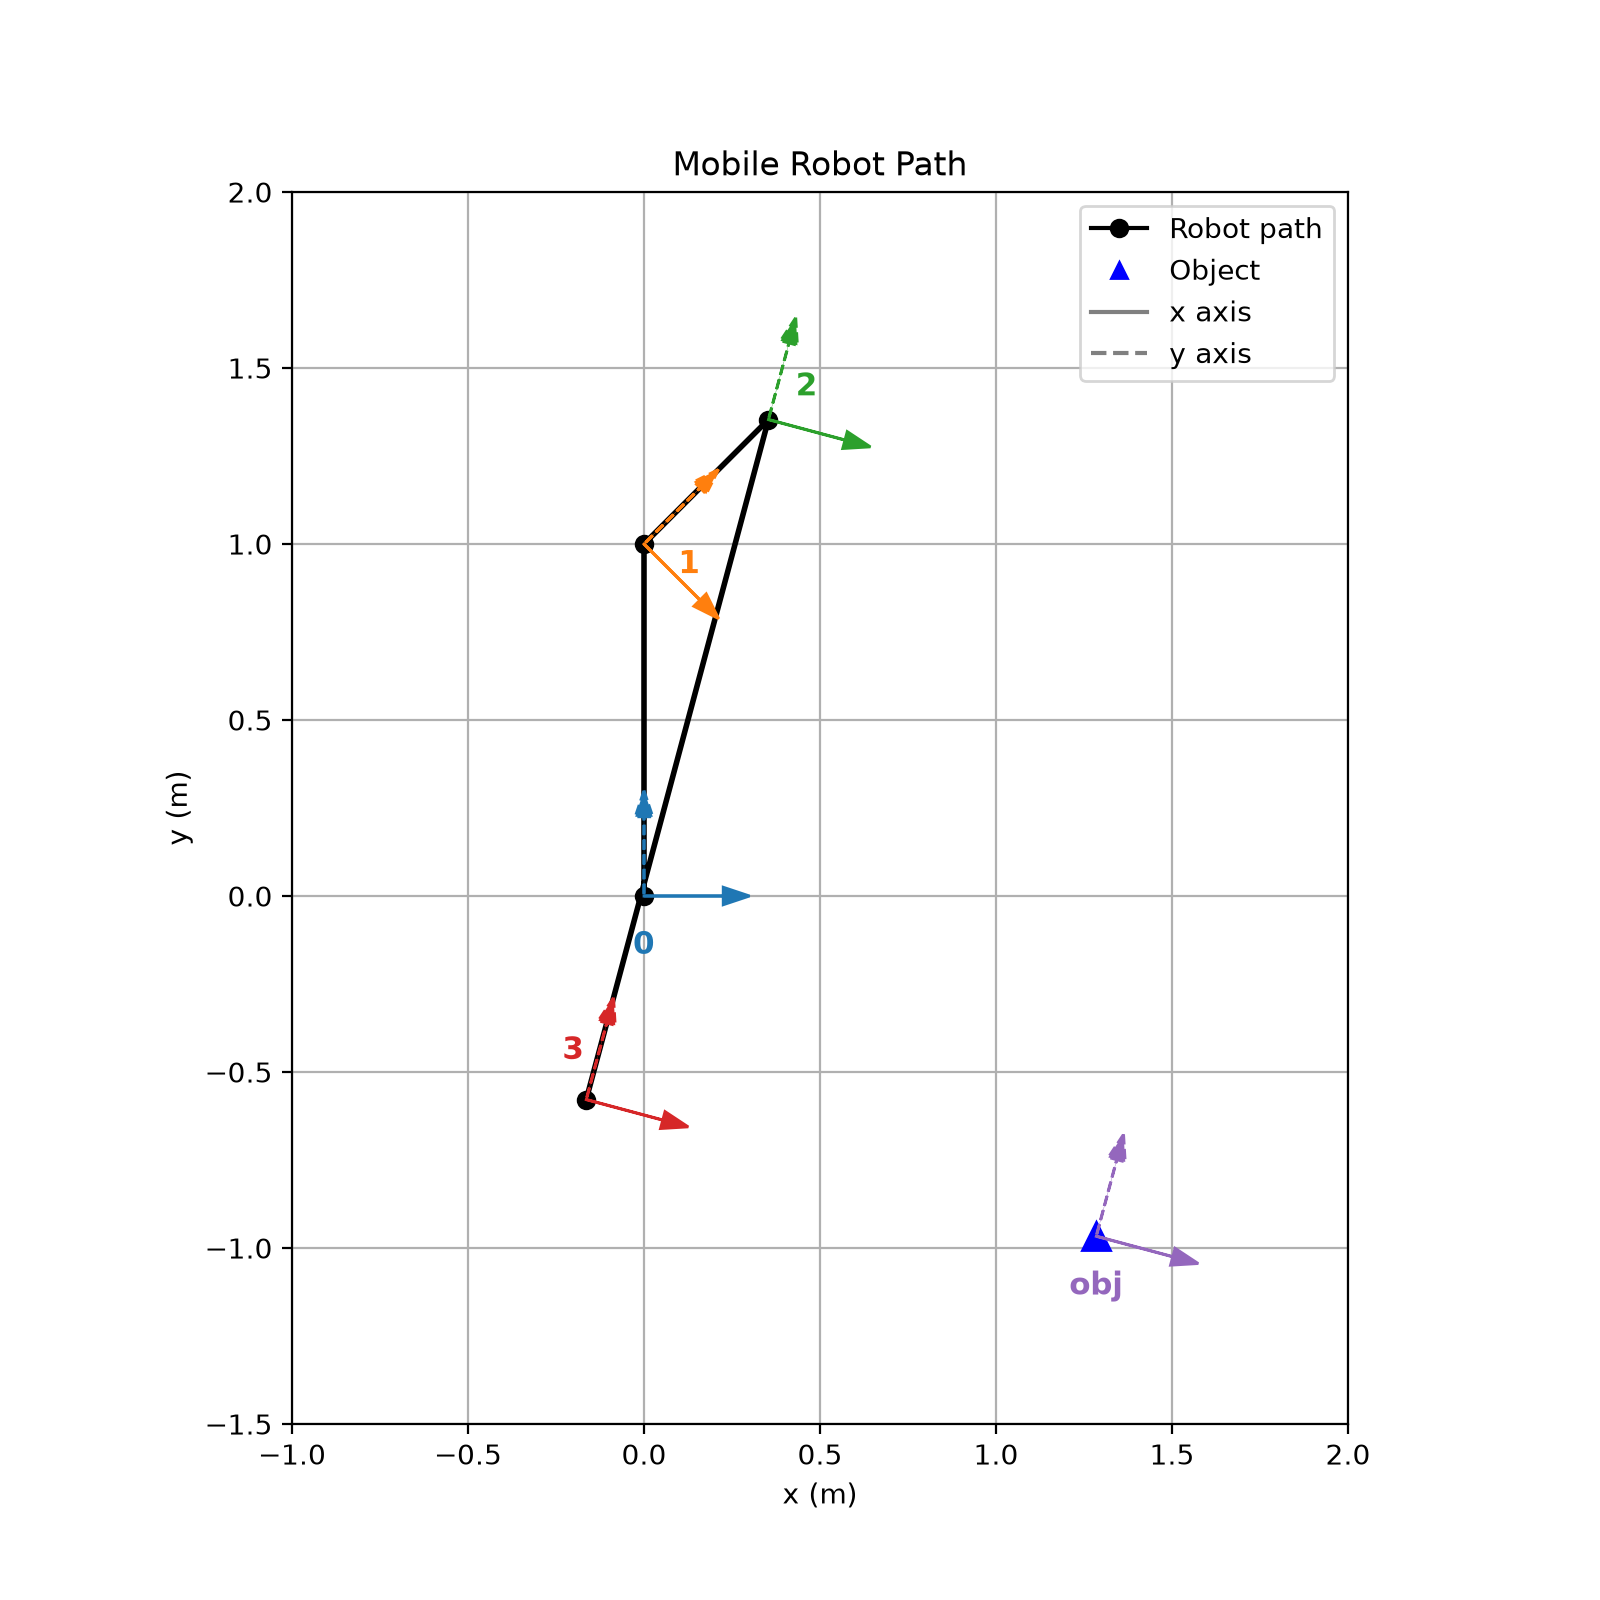
\includegraphics[width=0.55\linewidth]{Figures/Problem1A.png}
    \caption{Scaled path of the robot frame $\{r\}$ through frames $\{0\},\{1\},\{2\},\{3\}=\{\textrm{final}\}$, and the object frame $\{\textrm{obj}\}$.}
\end{figure}

\subsection*{Part (b): $^{0}\T_{\textrm{final}}$ as an Ordered Product of $\Trans(\cdot)$ and $\Rotz(\cdot)$}
Each motion is applied in the moving (body) frame, so the transforms are post-multiplied in the order executed:
\[
    ^{0}\T_{\textrm{final}} = \Trans\!\begin{pmatrix}0\\1\end{pmatrix}\Rotz(-45^\circ)\;\Trans\!\begin{pmatrix}0\\0.5\end{pmatrix}\Rotz(30^\circ)\;\Trans\!\begin{pmatrix}0\\-2\end{pmatrix}
\]

\subsection*{Part (c): $\prescript{0}{}{\T}_{\textrm{final}}$}
Writing the product as $^{0}\T_{\textrm{final}} = {}^{0}\T_1\,{}^{1}\T_2\,{}^{2}\T_3$:
\[
    \underbrace{\begin{bmatrix}\tfrac{\sqrt2}{2}&\tfrac{\sqrt2}{2}&0\\-\tfrac{\sqrt2}{2}&\tfrac{\sqrt2}{2}&1\\0&0&1\end{bmatrix}}_{^{0}\T_1}
    \underbrace{\begin{bmatrix}\tfrac{\sqrt3}{2}&-\tfrac12&0\\\tfrac12&\tfrac{\sqrt3}{2}&0.5\\0&0&1\end{bmatrix}}_{^{1}\T_2}
    \underbrace{\begin{bmatrix}1&0&0\\0&1&-2\\0&0&1\end{bmatrix}}_{^{2}\T_3}
\]
\begin{result}
\[
    ^{0}\T_{\textrm{final}} = \begin{bmatrix}0.9659 & 0.2588 & -0.1641 \\ -0.2588 & 0.9659 & -0.5782 \\ 0 & 0 & 1\end{bmatrix}
\]
\end{result}

\subsection*{Part (d): $\prescript{\textrm{final}}{}{\T}_{\textrm{obj}}$}
General form:
\[
    ^{F}\T_{\textrm{obj}} = \begin{bmatrix}^{F}\R_{\textrm{obj}} & ^{F}\dvec_{F\to\textrm{obj}} \\ \vec{0}^{T} & 1\end{bmatrix}
\]
The object is $1.5\,$m to the robot's right (i.e.\ along $\hat{\bm{x}}_{\textrm{final}}$) with the same orientation as $\{\textrm{final}\}$, so $^{F}\R_{\textrm{obj}}=\bm I$ and $^{F}\dvec_{F\to\textrm{obj}}=\begin{bmatrix}1.5\\0\end{bmatrix}$:
\begin{result}
\[
    ^{\textrm{final}}\T_{\textrm{obj}} = \begin{bmatrix}1 & 0 & 1.5 \\ 0 & 1 & 0 \\ 0 & 0 & 1\end{bmatrix}
\]
\end{result}

\subsection*{Part (e): $\prescript{\textrm{obj}}{}{\T}_{0}$}
First chain to the world frame:
\[
    ^{0}\T_{\textrm{obj}} = {}^{0}\T_{\textrm{final}}\cdot{}^{\textrm{final}}\T_{\textrm{obj}} = \begin{bmatrix}0.9659 & 0.2588 & 1.2848 \\ -0.2588 & 0.9659 & -0.9665 \\ 0 & 0 & 1\end{bmatrix}
\]
Then invert using $^{0}\T_{\textrm{obj}}^{-1} = \begin{bmatrix}{}^{0}\R_{\textrm{obj}}^{T} & -{}^{0}\R_{\textrm{obj}}^{T}\,{}^{0}\dvec_{0\to\textrm{obj}} \\ \vec{0}^{T} & 1\end{bmatrix}$:
\begin{result}
\[
    ^{\textrm{obj}}\T_{0} = \begin{bmatrix}0.9659 & -0.2588 & -1.4910 \\ 0.2588 & 0.9659 & 0.6010 \\ 0 & 0 & 1\end{bmatrix}
\]
\end{result}

% ====================================================
% PROBLEM 2
% ====================================================
\newpage
\section*{Problem 2}

\begin{statement}
Figure~\ref{fig:rpr} shows a three-link manipulator. The first joint is at the origin ${O}_0$ and rotates about $\prescript{0}{}{\hat{\bm{z}}}$ with an angle $\theta_0$. The first link has a length of $1\,$\unit{m}. The second link is prismatic and extends and contracts with length $a_1$, it is attached at a \SI{45}{\degree} rotation clockwise about the $\prescript{1}{}{\hat{\bm{z}}}$ direction. The third joint is again rotary and rotates relative to the second link by angle $\theta_2$. The third link has a length of $1\,$\unit{m}.
\end{statement}

\begin{figure}[H]
    \centering
    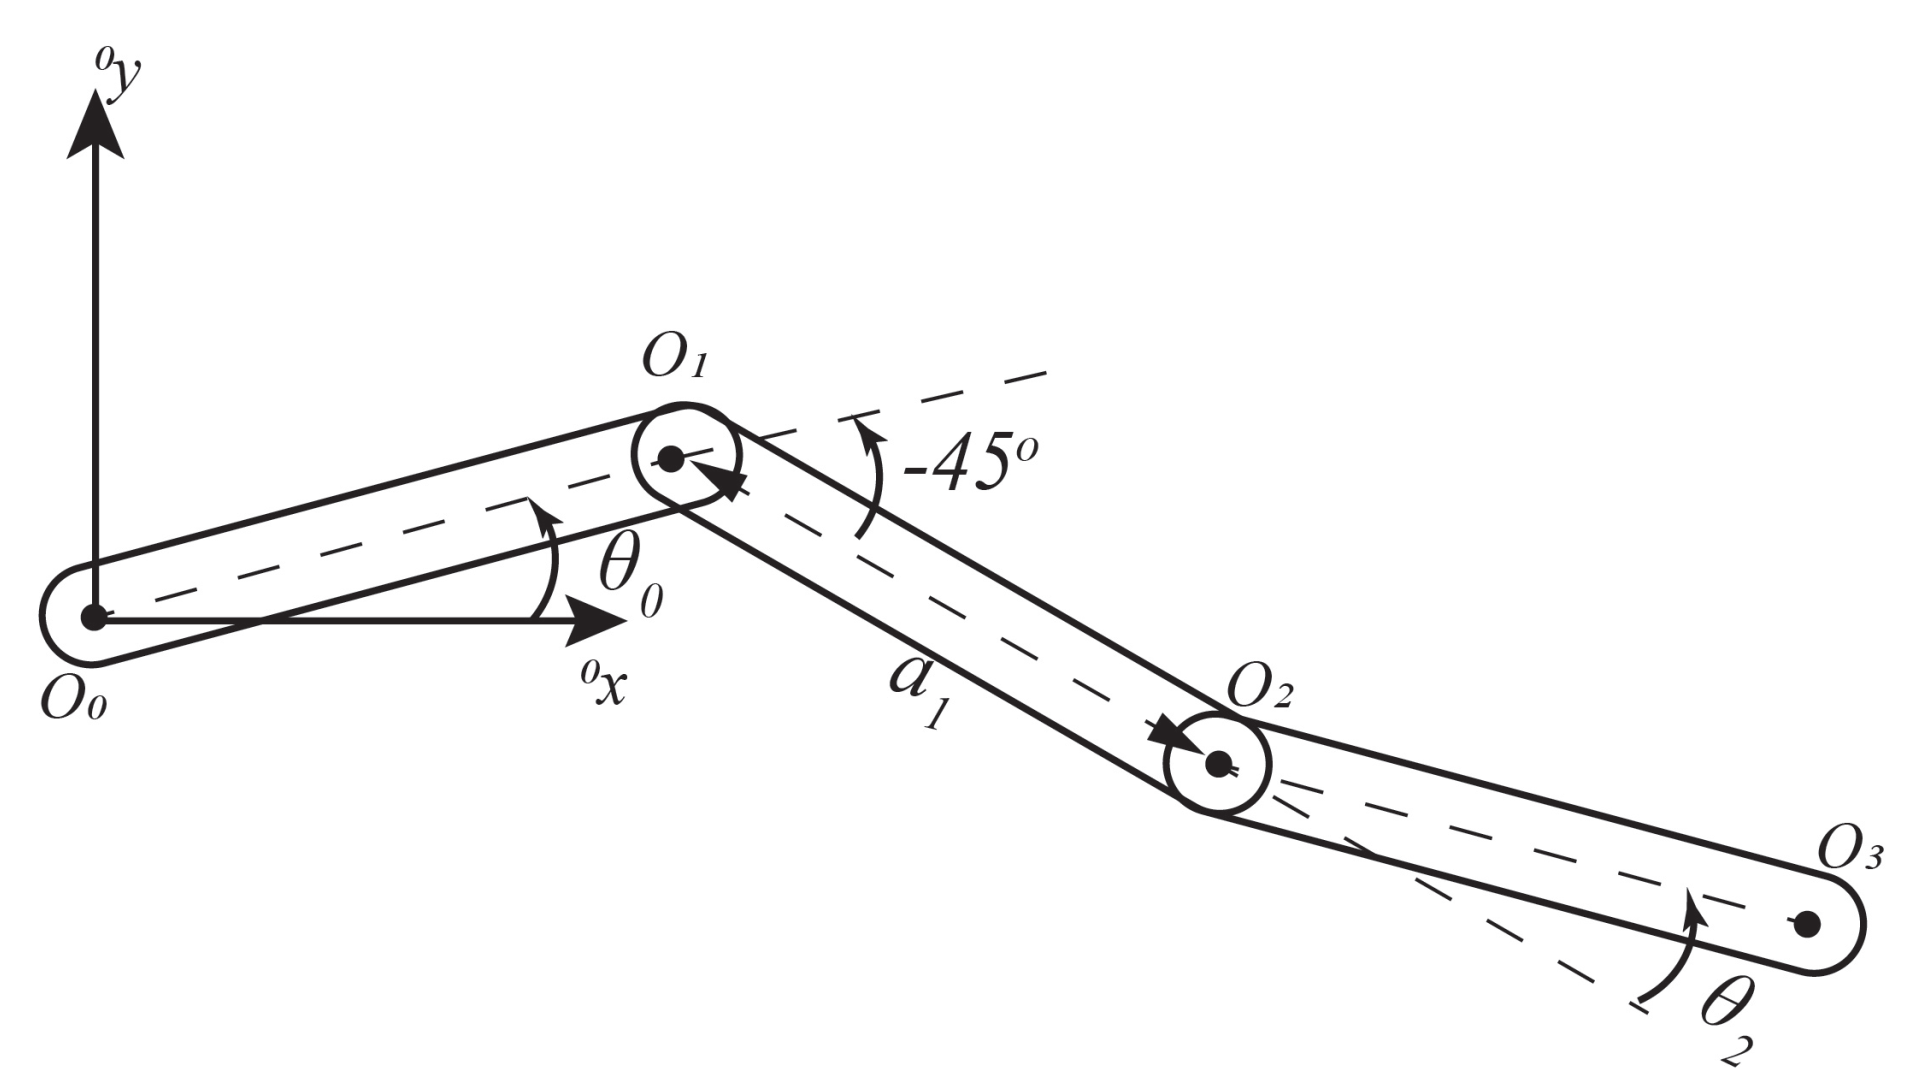
\includegraphics[width=0.6\linewidth]{Figures/RPR_manipulator.png}
    \caption{Three-link RPR manipulator.}
    \label{fig:rpr}
\end{figure}

\subsection*{Part (a): Manipulator Drawing ($\theta_0=\pi/4$, $a_1=0.5\,$m, $\theta_2=\pi/4$)}
\begin{figure}[H]
    \centering
    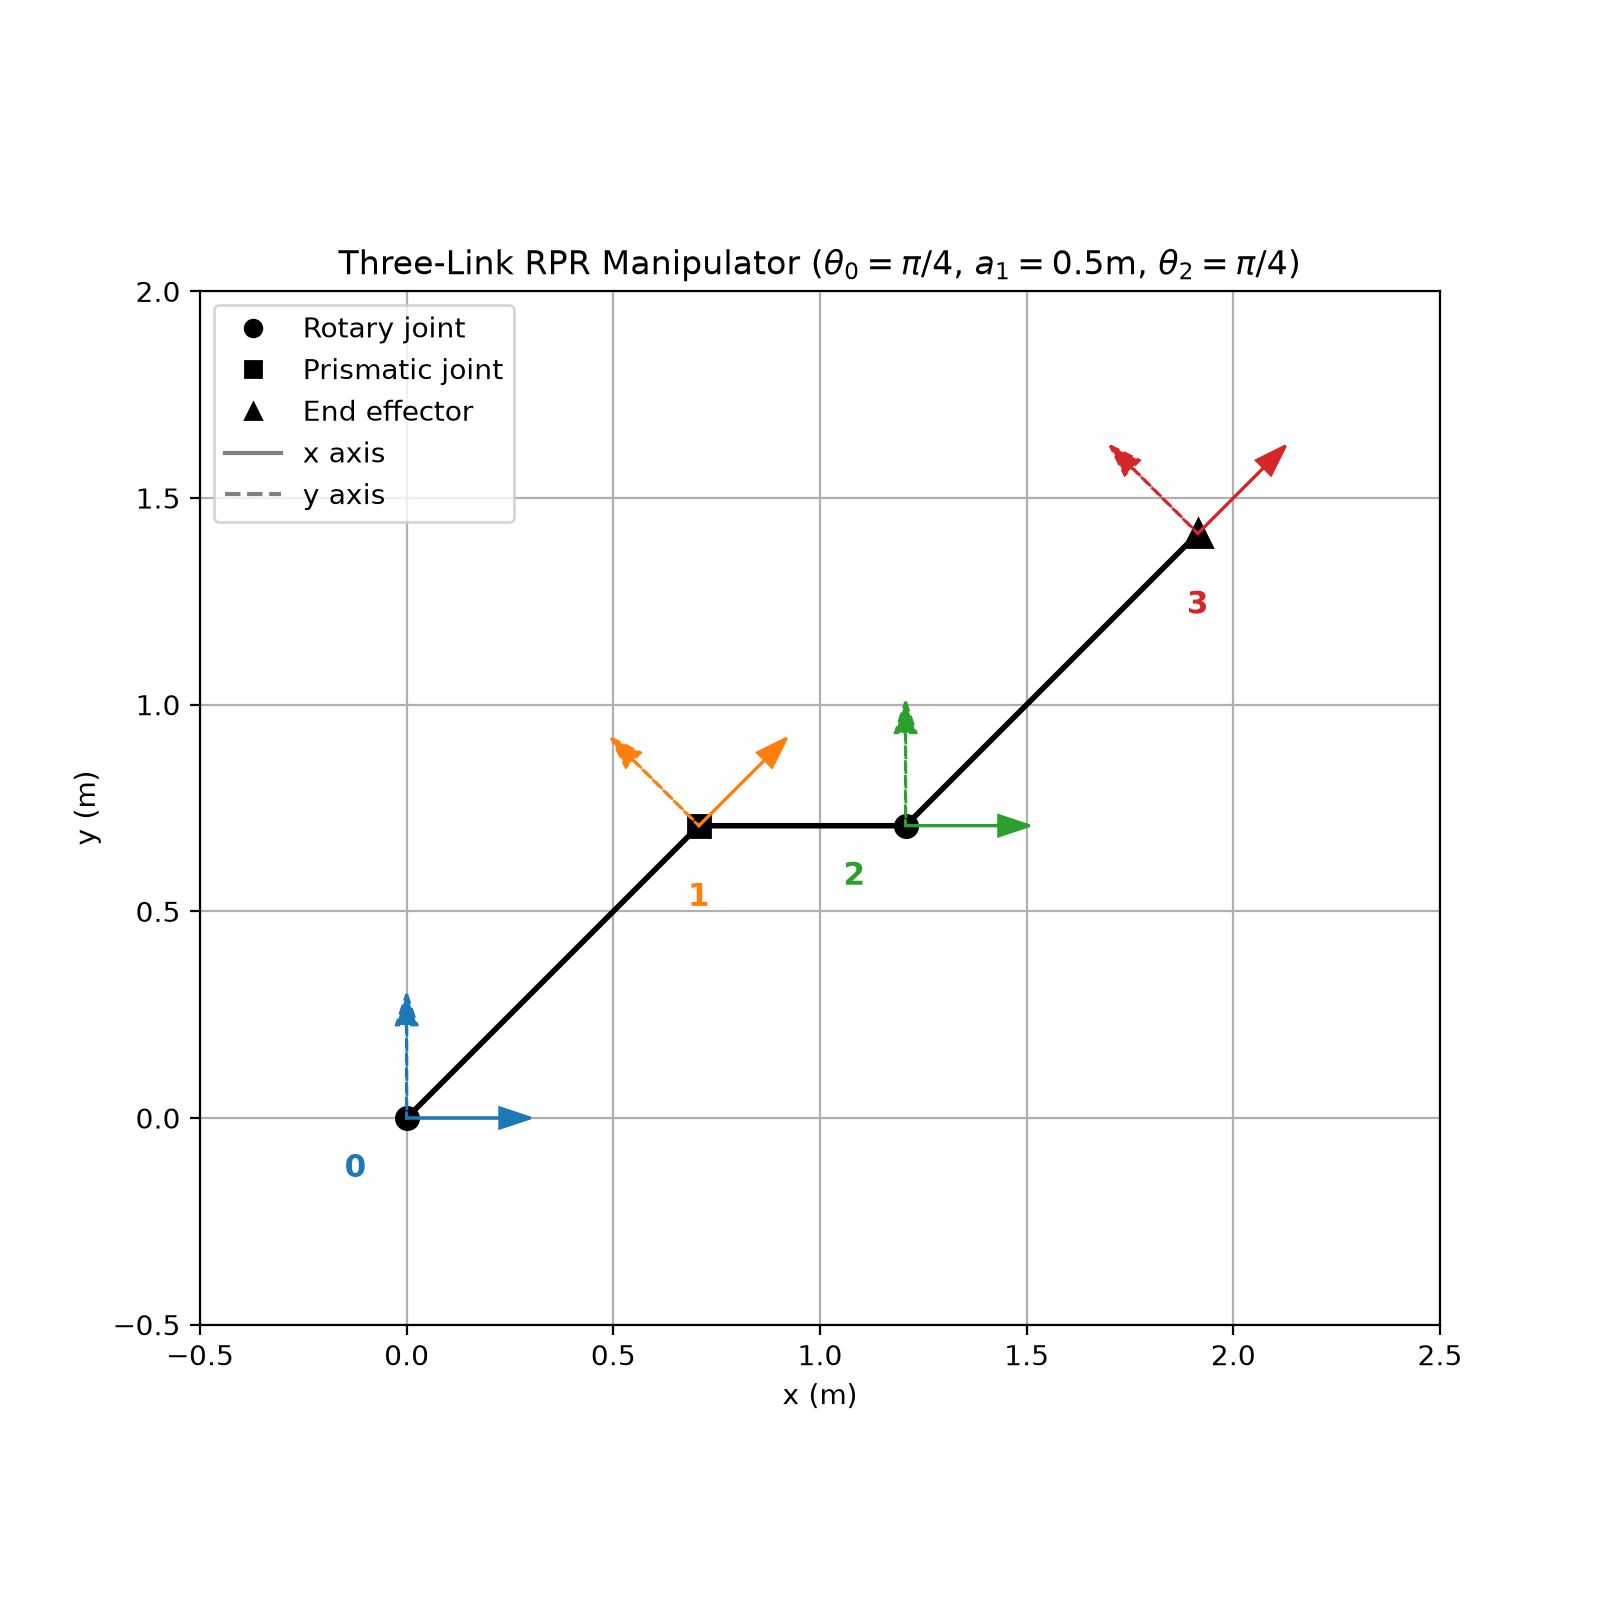
\includegraphics[width=0.55\linewidth]{Figures/Problem2A.png}
    \caption{RPR manipulator drawn to scale for $\theta_0=\pi/4$, $a_1=0.5\,$m, $\theta_2=\pi/4$.}
\end{figure}

\subsection*{Part (b): $\prescript{0}{}{\T}_{1}$}
\[
    ^{0}\T_1 = \begin{bmatrix}^{0}\R_1 & ^{0}\dvec_{01} \\ \vec 0^{T} & 1\end{bmatrix}, \qquad
    ^{0}\R_1 = \begin{bmatrix}c\theta_0 & -s\theta_0 \\ s\theta_0 & c\theta_0\end{bmatrix}
\]
Link 1 has length $1\,$m along $\hat{\bm x}_1$: $^{1}\dvec_{01} = 1\,{}^{1}\hat{\bm x}$, so $^{0}\dvec_{01} = 1c\theta_0\,\hat{\bm x} + 1s\theta_0\,\hat{\bm y}$.
\begin{result}
\[
    ^{0}\T_1 = \begin{bmatrix}c\theta_0 & -s\theta_0 & c\theta_0 \\ s\theta_0 & c\theta_0 & s\theta_0 \\ 0 & 0 & 1\end{bmatrix}
\]
\end{result}

\subsection*{Part (c): $\prescript{1}{}{\T}_{2}$}
Joint 1 is attached with a fixed $-45^\circ$ rotation about $^{1}\hat{\bm z}$:
\[
    ^{1}\T_2 = \begin{bmatrix}^{1}\R_2 & ^{1}\dvec_{12} \\ \vec 0^{T} & 1\end{bmatrix}, \qquad
    ^{1}\R_2 = \begin{bmatrix}\cos(-45^\circ) & -\sin(-45^\circ) \\ \sin(-45^\circ) & \cos(-45^\circ)\end{bmatrix} = \begin{bmatrix}\tfrac{\sqrt2}{2} & \tfrac{\sqrt2}{2} \\ -\tfrac{\sqrt2}{2} & \tfrac{\sqrt2}{2}\end{bmatrix}
\]
The prismatic link has length $a_1$ along $\hat{\bm x}_2$: $^{2}\dvec_{12} = a_1\,{}^{2}\hat{\bm x}$, so $^{1}\dvec_{12} = a_1\tfrac{\sqrt2}{2}\hat{\bm x} - a_1\tfrac{\sqrt2}{2}\hat{\bm y}$.
\begin{result}
\[
    ^{1}\T_2 = \begin{bmatrix}\tfrac{\sqrt2}{2} & \tfrac{\sqrt2}{2} & a_1\tfrac{\sqrt2}{2} \\ -\tfrac{\sqrt2}{2} & \tfrac{\sqrt2}{2} & -a_1\tfrac{\sqrt2}{2} \\ 0 & 0 & 1\end{bmatrix}
\]
\end{result}

\subsection*{Part (d): $\prescript{2}{}{\T}_{3}$}
\[
    ^{2}\T_3 = \begin{bmatrix}^{2}\R_3 & ^{2}\dvec_{23} \\ \vec 0^{T} & 1\end{bmatrix}, \qquad
    ^{2}\R_3 = \begin{bmatrix}c\theta_2 & -s\theta_2 \\ s\theta_2 & c\theta_2\end{bmatrix}
\]
Link 3 has length $1\,$m along $\hat{\bm x}_3$: $^{3}\dvec_{23} = 1\,{}^{3}\hat{\bm x}$, so $^{2}\dvec_{23} = c\theta_2\,\hat{\bm x} + s\theta_2\,\hat{\bm y}$.
\begin{result}
\[
    ^{2}\T_3 = \begin{bmatrix}c\theta_2 & -s\theta_2 & c\theta_2 \\ s\theta_2 & c\theta_2 & s\theta_2 \\ 0 & 0 & 1\end{bmatrix}
\]
\end{result}

\subsection*{Part (e): $\prescript{0}{}{\T}_{3}$}
\[
    ^{0}\T_3 = {}^{0}\T_1\,{}^{1}\T_2\,{}^{2}\T_3 =
    \begin{bmatrix}c\theta_0 & -s\theta_0 & c\theta_0 \\ s\theta_0 & c\theta_0 & s\theta_0 \\ 0 & 0 & 1\end{bmatrix}
    \begin{bmatrix}\tfrac{\sqrt2}{2} & \tfrac{\sqrt2}{2} & a_1\tfrac{\sqrt2}{2} \\ -\tfrac{\sqrt2}{2} & \tfrac{\sqrt2}{2} & -a_1\tfrac{\sqrt2}{2} \\ 0 & 0 & 1\end{bmatrix}
    \begin{bmatrix}c\theta_2 & -s\theta_2 & c\theta_2 \\ s\theta_2 & c\theta_2 & s\theta_2 \\ 0 & 0 & 1\end{bmatrix}
\]
Since $\R(\theta_0)\R(-45^\circ)\R(\theta_2)=\R(\theta_0-45^\circ+\theta_2)$, the product simplifies to:
\begin{result}
\[
    ^{0}\T_3 = \begin{bmatrix}
        c(\theta_0-45^\circ+\theta_2) & -s(\theta_0-45^\circ+\theta_2) & c\theta_0 + a_1c(\theta_0-45^\circ) + c(\theta_0-45^\circ+\theta_2) \\
        s(\theta_0-45^\circ+\theta_2) & c(\theta_0-45^\circ+\theta_2) & s\theta_0 + a_1s(\theta_0-45^\circ) + s(\theta_0-45^\circ+\theta_2) \\
        0 & 0 & 1
    \end{bmatrix}
\]
\end{result}

% ====================================================
% PROBLEM 3
% ====================================================
\newpage
\section*{Problem 3}

\begin{statement}
Figure~\ref{fig:path} shows the path of a mobile robot. The displacements are given by:
\[
    \prescript{0}{}{\dvec}_{01} = \begin{bmatrix}2\\1\end{bmatrix}, \quad
    \prescript{1}{}{\dvec}_{12} = \begin{bmatrix}0\\0\end{bmatrix}, \quad
    \prescript{2}{}{\dvec}_{23} = \begin{bmatrix}2\\0\end{bmatrix}, \quad
    \prescript{3}{}{\dvec}_{34} = \begin{bmatrix}0\\0\end{bmatrix}, \quad
    \prescript{4}{}{\dvec}_{45} = \begin{bmatrix}0\\3\end{bmatrix}.
\]
\end{statement}

\begin{figure}[H]
    \centering
    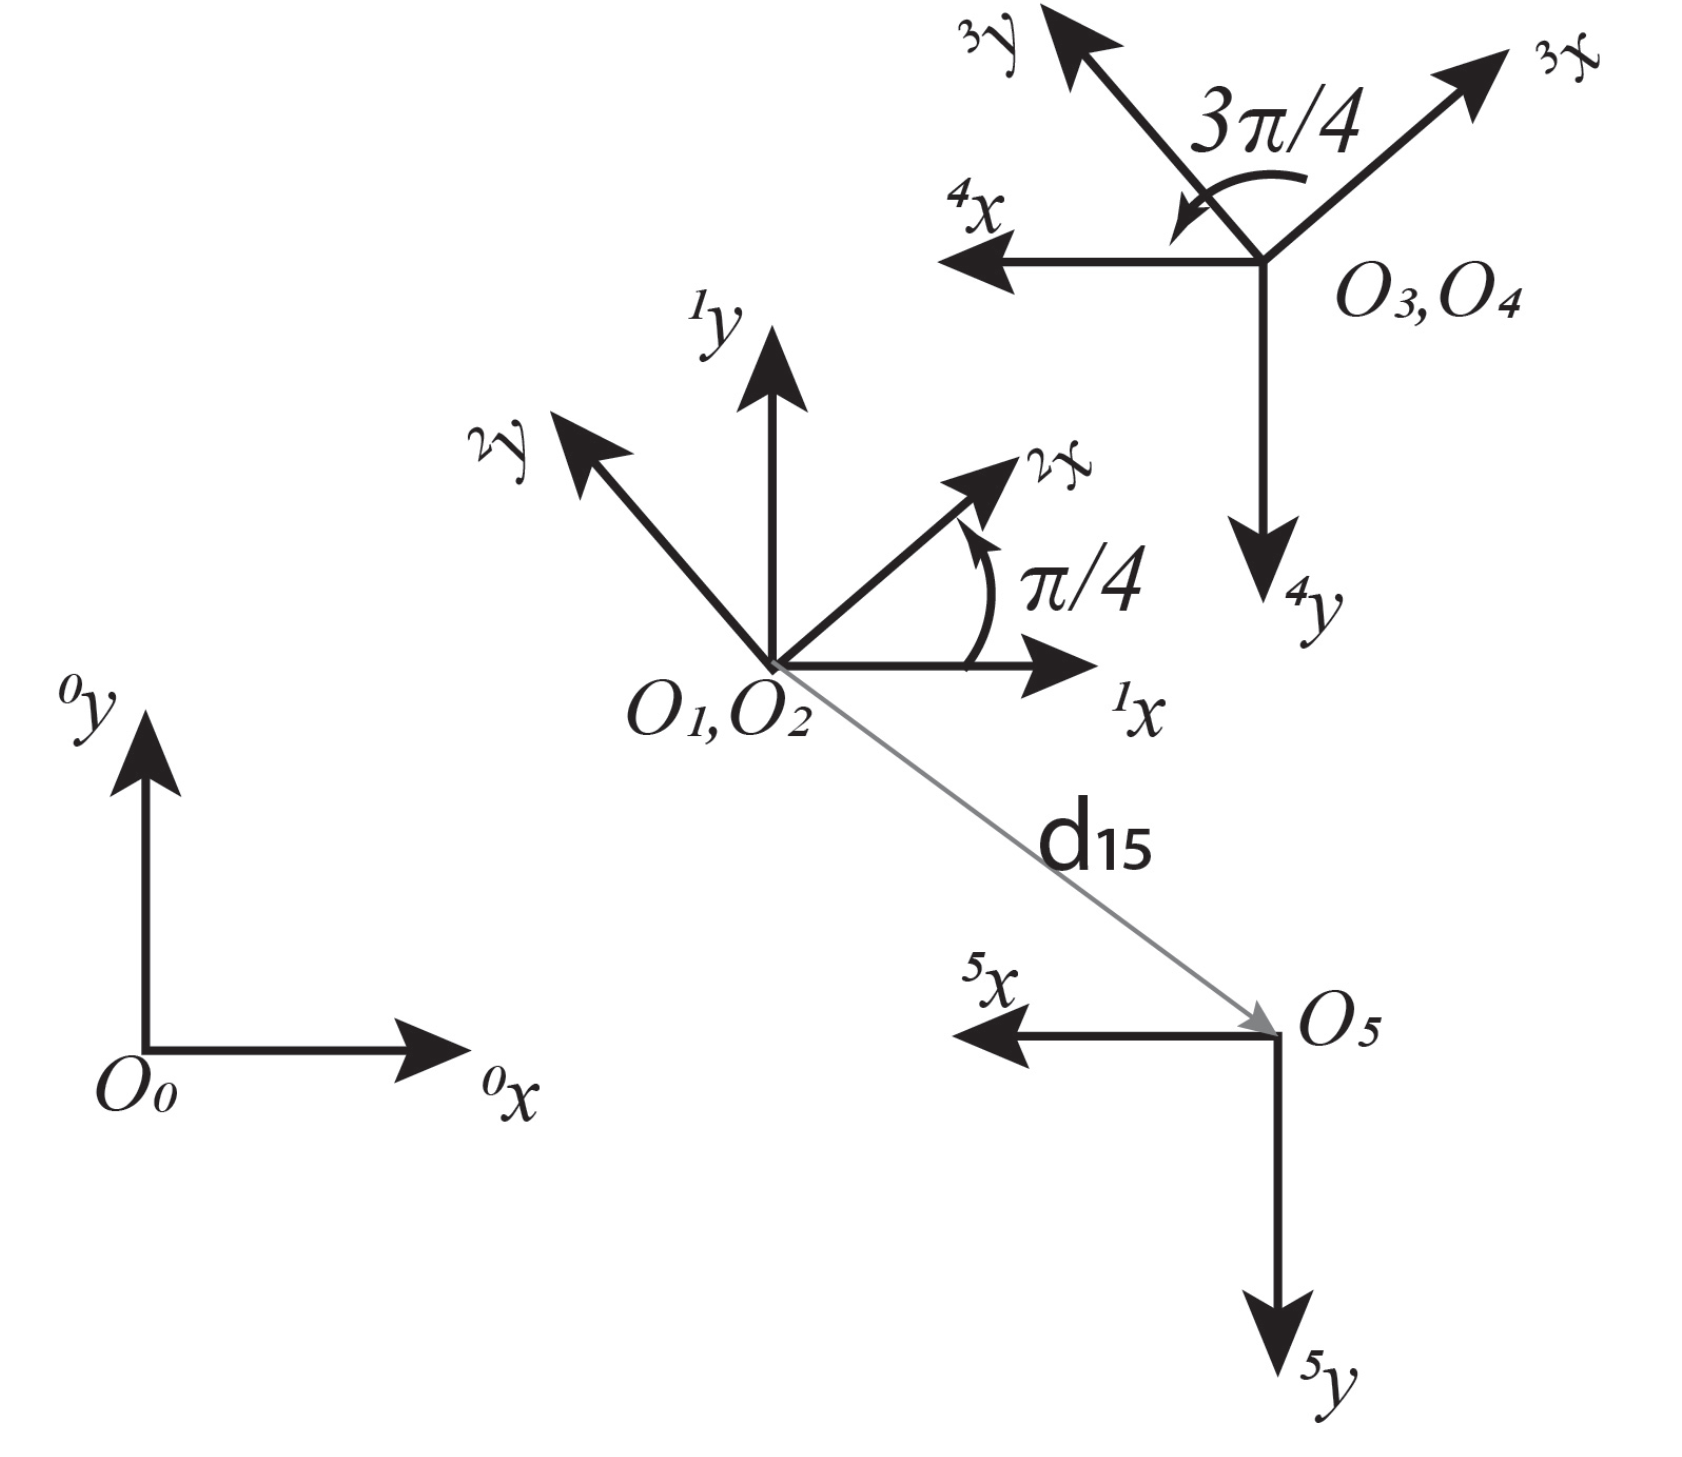
\includegraphics[width=0.5\linewidth]{Figures/path_mobile_robot.png}
    \caption{Path of mobile robot.}
    \label{fig:path}
\end{figure}

\subsection*{Part (a): $\prescript{0}{}{\T}_{1}$}
\[
    ^{0}\T_1 = \begin{bmatrix}^{0}\R_1 & ^{0}\dvec_{01} \\ \vec 0^{T} & 1\end{bmatrix}, \qquad {}^{0}\R_1 = \bm I, \qquad {}^{0}\dvec_{01}=\begin{bmatrix}2\\1\end{bmatrix}
\]
\begin{result}
\[
    ^{0}\T_1 = \begin{bmatrix}1 & 0 & 2 \\ 0 & 1 & 1 \\ 0 & 0 & 1\end{bmatrix}
\]
\end{result}

\subsection*{Part (b): $\prescript{1}{}{\T}_{2}$}
\[
    ^{1}\T_2 = \begin{bmatrix}^{1}\R_2 & ^{1}\dvec_{12} \\ \vec 0^{T} & 1\end{bmatrix}, \qquad ^{1}\R_2=\begin{bmatrix}c\theta&-s\theta\\s\theta&c\theta\end{bmatrix},\ \theta=\pi/4, \qquad {}^{1}\dvec_{12}=\begin{bmatrix}0\\0\end{bmatrix}
\]
\begin{result}
\[
    ^{1}\T_2 = \begin{bmatrix}\tfrac{\sqrt2}{2} & -\tfrac{\sqrt2}{2} & 0 \\ \tfrac{\sqrt2}{2} & \tfrac{\sqrt2}{2} & 0 \\ 0 & 0 & 1\end{bmatrix}
\]
\end{result}

\subsection*{Part (c): $\prescript{2}{}{\T}_{3}$}
$^{2}\R_3=\bm I$ since frame $\{3\}$'s axes are parallel to frame $\{2\}$'s (Fig.~\ref{fig:path}), with $^{2}\dvec_{23}=\begin{bmatrix}2\\0\end{bmatrix}$:
\begin{result}
\[
    ^{2}\T_3 = \begin{bmatrix}1 & 0 & 2 \\ 0 & 1 & 0 \\ 0 & 0 & 1\end{bmatrix}
\]
\end{result}

\subsection*{Part (d): $\prescript{3}{}{\T}_{4}$}
Frames $\{3\}$ and $\{4\}$ are coincident, related by a $3\pi/4$ rotation: $s,c(3\pi/4)=\tfrac{\sqrt2}{2},-\tfrac{\sqrt2}{2}$.
\begin{result}
\[
    ^{3}\T_4 = \begin{bmatrix}-\tfrac{\sqrt2}{2} & -\tfrac{\sqrt2}{2} & 0 \\ \tfrac{\sqrt2}{2} & -\tfrac{\sqrt2}{2} & 0 \\ 0 & 0 & 1\end{bmatrix}
\]
\end{result}

\subsection*{Part (e): $\prescript{4}{}{\T}_{5}$}
\begin{result}
\[
    ^{4}\T_5 = \begin{bmatrix}1 & 0 & 0 \\ 0 & 1 & 3 \\ 0 & 0 & 1\end{bmatrix}
\]
\end{result}

\subsection*{Part (f): $\prescript{0}{}{\T}_{5}$}
\[
    ^{0}\T_5 = {}^{0}\T_1\,{}^{1}\T_2\,{}^{2}\T_3\,{}^{3}\T_4\,{}^{4}\T_5
\]
\begin{result}
\[
    ^{0}\T_5 = \begin{bmatrix}-1 & 0 & 3.41 \\ 0 & -1 & -0.59 \\ 0 & 0 & 1\end{bmatrix}
\]
\end{result}

\subsection*{Part (g): $\prescript{0}{}{\dvec}_{05}$}
\begin{result}
\[
    ^{0}\dvec_{05} = \begin{bmatrix}3.41\\-0.59\end{bmatrix}
\]
\end{result}

\subsection*{Part (h): $\prescript{0}{}{\R}_{5}$}
\begin{result}
\[
    ^{0}\R_5 = \begin{bmatrix}-1 & 0 \\ 0 & -1\end{bmatrix}
\]
\end{result}

\subsection*{Part (i): Displacement from Origin 1 to Origin 5, Expressed in Frame 5}

\paragraph{(I) Homogeneous-transformation equation for $\dvec_{15}$ in frame 5.}
The displacement is found via $^{5}\dvec_{51}$, obtained by mapping $^{0}\dvec_{01}$ through $^{0}\T_5^{-1}$, then negated:
\[
    ^{0}\T_5^{-1} = \begin{bmatrix}^{0}\R_5^{-1} & -{}^{0}\R_5^{-1}\,{}^{0}\dvec_{05} \\ \vec 0^{T} & 1\end{bmatrix}, \qquad
    \begin{bmatrix}^{5}\dvec_{51}\\1\end{bmatrix} = {}^{0}\T_5^{-1}\begin{bmatrix}^{0}\dvec_{01}\\1\end{bmatrix}, \qquad {}^{5}\dvec_{15} = -{}^{5}\dvec_{51}
\]

\paragraph{(II) Numerical value.}
Since $^{0}\R_5=-\bm I$ satisfies $\R^2=\bm I$ and $\R\dvec_{05}+\dvec_{05}=\vec 0$, $^{0}\T_5$ is an involution, so $^{0}\T_5^{-1}={}^{0}\T_5$ numerically. The matrix below is not a copy-paste of the forward transform; it is the correct inverse:
\[
    ^{0}\T_5^{-1} = \begin{bmatrix}-1 & 0 & 3.41 \\ 0 & -1 & -0.59 \\ 0 & 0 & 1\end{bmatrix}, \qquad
    ^{5}\dvec_{51} = {}^{0}\T_5^{-1}\begin{bmatrix}2\\1\\1\end{bmatrix} = \begin{bmatrix}1.41\\-1.59\end{bmatrix}
\]
\begin{result}
\[
    ^{5}\dvec_{15} = \begin{bmatrix}-1.41\\1.59\end{bmatrix}
\]
\end{result}

% ====================================================
% PROBLEM 4
% ====================================================
\newpage
\section*{Problem 4}

\begin{statement}
Determine if the following matrices are rotations and explain why or why not.
\end{statement}

\subsection*{Part (a)}
\[
    \begin{bmatrix}
        0 & 1 & 0 \\
        1 & 0 & 0 \\
        0 & 0 & 1
    \end{bmatrix}
\]
Expanding along the first row: $\det = 0\cdot(\cdots) - 1\cdot(1\cdot1-0\cdot0) + 0\cdot(\cdots) = -1$.
\begin{result}
$\det=-1\neq1$, so this is \textbf{not a rotation} (it is a reflection).
\end{result}

\subsection*{Part (b)}
\[
    \begin{bmatrix}
        0 & 1 & 0 \\
        1 & 0 & 0 \\
        0 & 0 & -1
    \end{bmatrix}
\]
Each column has unit norm, columns are mutually orthogonal ($\bm c_i\cdot\bm c_j=0$), and $\det(\bm B)=1$.
\begin{result}
\textbf{Yes, this is a rotation.}
\end{result}

\subsection*{Part (c)}
\[
    \begin{bmatrix}
        -0.254 & 0.087 & -0.963 \\
        0.967 & 0.0169 & -0.253 \\
        -0.00572 & -0.996 & -0.0884
    \end{bmatrix}
\]
$\lVert\bm c_i\rVert_2=1$, $\bm c_i\cdot\bm c_j=0$, and $\det(\bm C)=1$.
\begin{result}
\textbf{Yes, this is a rotation.}
\end{result}

\subsection*{Part (d)}
\[
    \begin{bmatrix}
        0.546 & 0.0719 & -1.47 \\
        0.814 & -0.696 & -0.0502 \\
        -1.23 & -0.813 & 0.474
    \end{bmatrix}
\]
$\lVert\bm c_i\rVert_2\neq1$ (e.g.\ entries such as $-1.47$ and $-1.23$ already exceed unit magnitude).
\begin{result}
\textbf{Not a rotation.}
\end{result}

% ====================================================
% PROBLEM 5
% ====================================================
\newpage
\section*{Problem 5}

\begin{statement}
Complete the below rotation matrices. How do you know it is correct?
\end{statement}

\subsection*{Part (a)}
\[
    \begin{bmatrix}
        0 & 0 & ? \\
        0 & 1 & ? \\
        1 & 0 & ?
    \end{bmatrix}
\]
For a valid rotation the columns form a right-handed orthonormal set, so $\bm c_3 = \bm c_1\times\bm c_2 = \begin{bmatrix}0\\0\\1\end{bmatrix}\times\begin{bmatrix}0\\1\\0\end{bmatrix} = \begin{bmatrix}-1\\0\\0\end{bmatrix}$.
\begin{result}
\[
    \begin{bmatrix}
        0 & 0 & -1 \\
        0 & 1 & 0 \\
        1 & 0 & 0
    \end{bmatrix}
\]
This is correct because $\bm c_3=\bm c_1\times\bm c_2$ guarantees unit norm, mutual orthogonality, and $\det=+1$.
\end{result}

\subsection*{Part (b)}
\[
    \begin{bmatrix}
        -1 & ? & ? \\
        ? & 1 & ? \\
        ? & ? & ?
    \end{bmatrix}
\]
With $\bm c_1=\begin{bmatrix}-1\\0\\0\end{bmatrix}$, $\bm c_2=\begin{bmatrix}0\\1\\0\end{bmatrix}$: $\bm c_3=\bm c_1\times\bm c_2=\begin{bmatrix}0\\0\\-1\end{bmatrix}$.
\begin{result}
\[
    \begin{bmatrix}
        -1 & 0 & 0 \\
        0 & 1 & 0 \\
        0 & 0 & -1
    \end{bmatrix}
\]
Correct by the same right-hand-rule / orthonormality argument as part (a).
\end{result}

\subsection*{Part (c)}
\[
    \begin{bmatrix}
        0.3698 & ? & 0.8665 \\
        -0.9276 & ? & 0.324 \\
        -0.05236 & ? & 0.3797
    \end{bmatrix}
\]
Here $\bm c_1,\bm c_3$ are given, so $\bm c_2 = \bm c_3\times\bm c_1$:
\[
    \bm c_2 = \begin{bmatrix}0.8665\\0.324\\0.3797\end{bmatrix}\times\begin{bmatrix}0.3698\\-0.9276\\-0.05236\end{bmatrix} = \begin{bmatrix}0.3352\\0.1858\\-0.9235\end{bmatrix}
\]
\begin{result}
\[
    \begin{bmatrix}
        0.3698 & 0.3352 & 0.8665 \\
        -0.9276 & 0.1858 & 0.324 \\
        -0.05236 & -0.9235 & 0.3797
    \end{bmatrix}
\]
Correct since $\bm c_2=\bm c_3\times\bm c_1$ reproduces a right-handed orthonormal column set.
\end{result}

\subsection*{Part (d)}
\[
    \begin{bmatrix}
        ? & 0.1166 & ? \\
        -0.2039 & ? & 0.2153 \\
        ? & ? & -0.3672
    \end{bmatrix}
\]
With five unknowns, the cross-product shortcut does not apply directly since no column or row is fully known; the remaining entries were solved numerically (in Python) by enforcing the three defining properties of a rotation matrix: $\lVert\bm c_i\rVert_2=1$, $\bm c_i\cdot\bm c_j=0$ for $i\neq j$, and $\det=1$. These constraints have a sign ambiguity, so two completions are admissible:
\[
    \R = \begin{bmatrix}
        -0.4094 & 0.1166 & -0.9049 \\
        -0.2039 & 0.9550 & 0.2153 \\
        0.8893 & 0.2727 & -0.3672
    \end{bmatrix}
    \qquad\text{or}\qquad
    \R' = \begin{bmatrix}
        0.4094 & 0.1166 & 0.9049 \\
        -0.2039 & -0.9550 & 0.2153 \\
        0.8893 & -0.2727 & -0.3672
    \end{bmatrix}
\]
\begin{result}
$\R$ above is one of two admissible completions (the other, $\R'$ above, corresponds to the opposite sign of $a_{22}$, which then flips $a_{11}$, $a_{13}$, and $a_{32}$), and both are verified correct by satisfying unit column norms, mutual orthogonality, and $\bm c_1\times\bm c_2=\bm c_3$ (so $\det=+1$) while exactly reproducing the four given entries, meaning those entries alone do not determine a unique rotation matrix.
\end{result}

% ====================================================
% APPENDIX A: PYTHON CODE
% ====================================================
\newpage
\section*{Appendix A: Python Code}

\subsection*{Problem 1: Path and Frame Plot}
\lstinputlisting[caption={Problem 1.py: generates the scaled path drawing in Fig.~1.}]{"../Code/Problem 1.py"}

\newpage
\subsection*{Problem 2: Manipulator Plot}
\lstinputlisting[caption={Problem 2.py: generates the scaled manipulator drawing in Fig.~2.}]{"../Code/Problem 2.py"}

% ====================================================
% APPENDIX B: HAND CALCULATIONS
% ====================================================
\newpage
\section*{Appendix B: Hand Calculations}

\begin{fixnote}
\textbf{Corrections made when typing up the hand calcs below:}
\begin{enumerate}[leftmargin=1.2em, itemsep=4pt]
    \item \textbf{Problem 1(b), page 18:} the second rotation was written as $\Rotz(15^\circ)$, but the problem statement specifies a $30^\circ$ counter-clockwise turn, and the numeric matrix used in part (c) on the same page is built from $\cos 30^\circ=\tfrac{\sqrt3}{2}$, $\sin30^\circ=\tfrac12$, so $\Rotz(30^\circ)$ is what was actually (correctly) carried through the rest of the problem. Typed up as $\Rotz(30^\circ)$.
    \item \textbf{Problem 1(e), page 19:} the boxed $^{\textrm{obj}}\T_0$ had the rotation block negated ($-{}^{0}\R_{\textrm{obj}}^{T}$ used for the whole matrix rather than just the translation term), giving $\begin{bmatrix}-0.9659&0.2588\\-0.2588&-0.9659\end{bmatrix}$ and a translation of $(-1.4556,\,0.6105)$. Since $\{\textrm{obj}\}$ shares its orientation with $\{\textrm{final}\}$, $^{0}\R_{\textrm{obj}}=\R(-15^\circ)$, so $^{\textrm{obj}}\R_0={}^{0}\R_{\textrm{obj}}^{T}=\R(15^\circ)=\begin{bmatrix}0.9659&-0.2588\\0.2588&0.9659\end{bmatrix}$ (positive diagonal), with translation $-{}^{0}\R_{\textrm{obj}}^{T}\,{}^{0}\dvec_{0\to\textrm{obj}}\approx(-1.4910,\,0.6010)$. Typed up with the corrected values.
    \item \textbf{Problem 2(b), page 20:} the boxed $^{0}\T_1$ had $s\theta_0$ in the (2,2) entry instead of $c\theta_0$, a copy slip, since the correct $\cos\theta_0$ pattern is shown directly above it (in $^{0}\R_1$ on the same page) and is used consistently in the part (e) derivation on page 23. Typed up with $c\theta_0$.
\end{enumerate}
\end{fixnote}

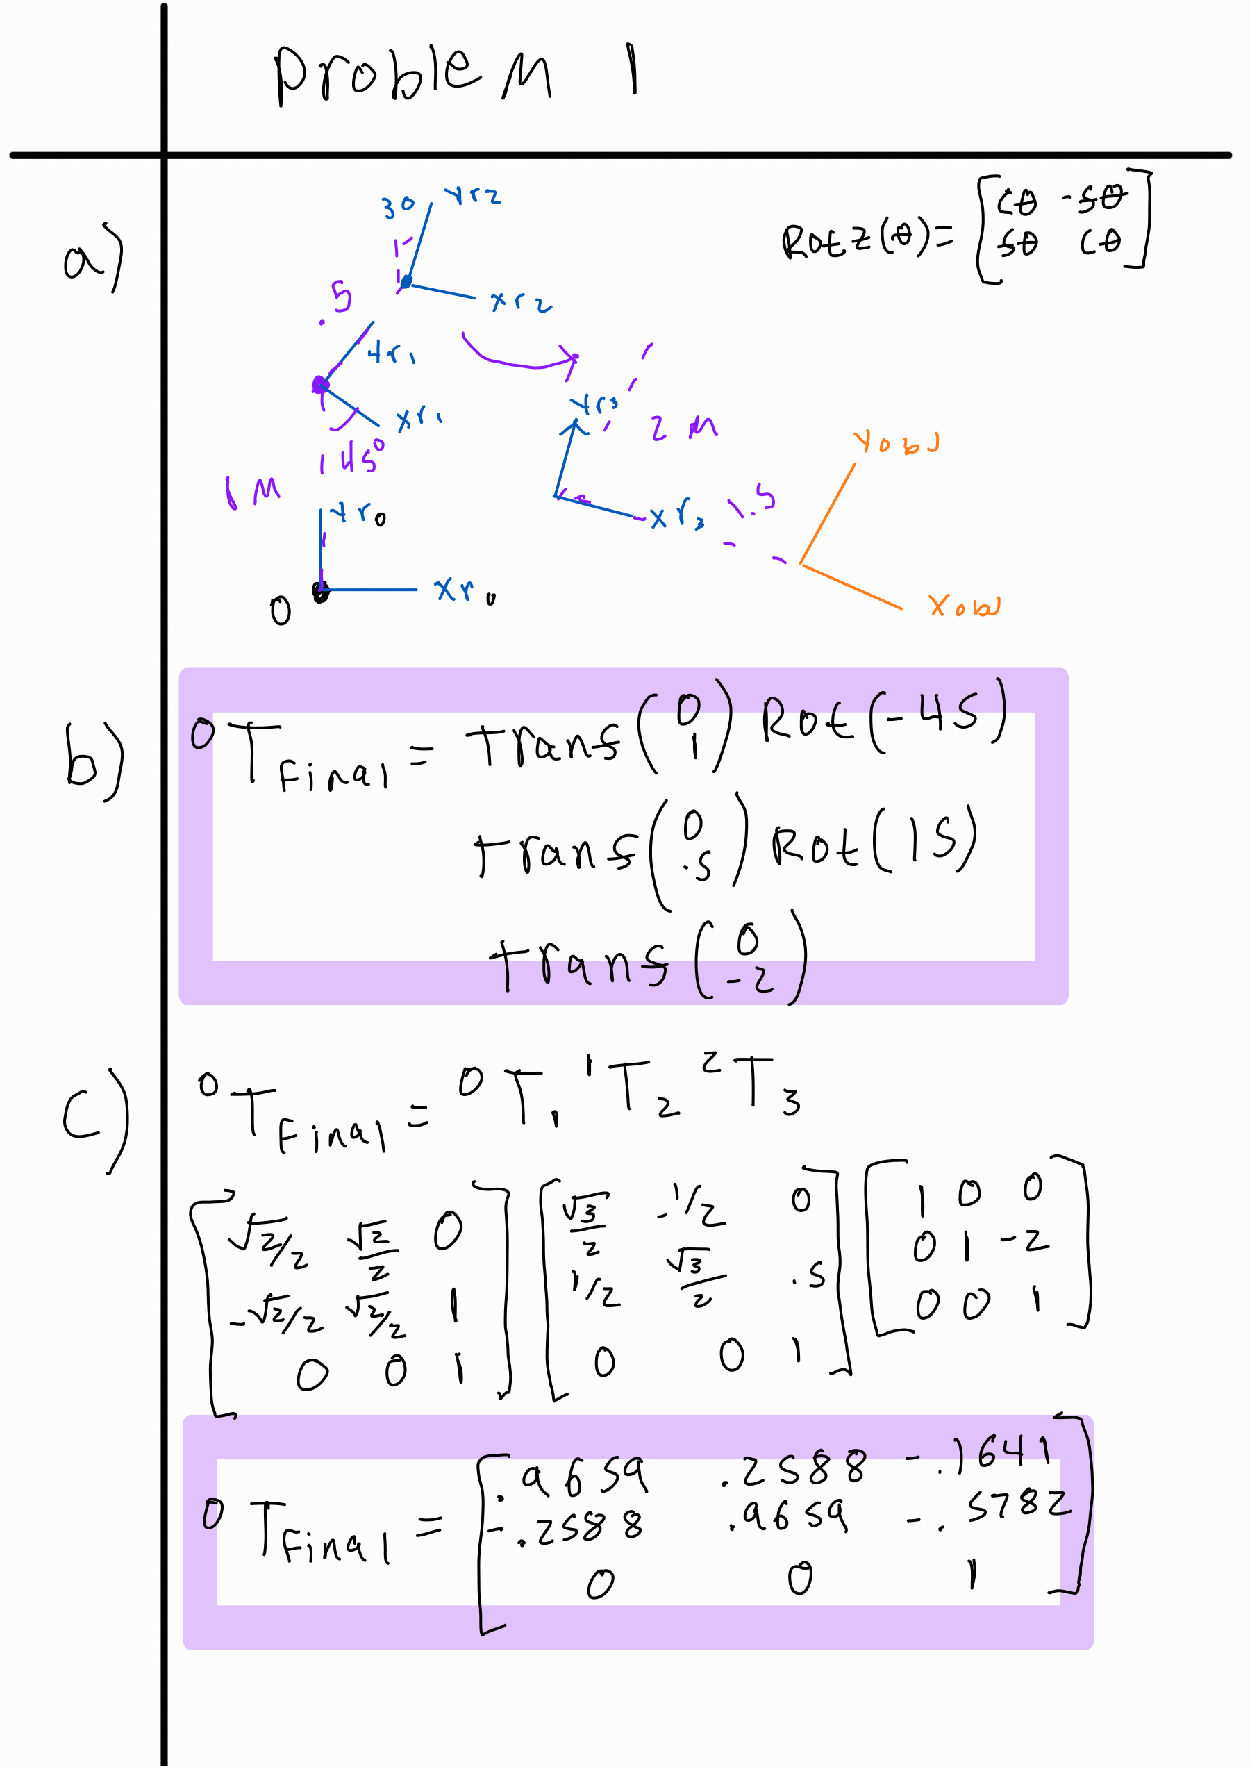
\includepdf[pages=-, pagecommand={\thispagestyle{plain}}, scale=0.9]{../Homework 1_hand_calcs.pdf}

\end{document}
